\documentclass[twocolumn]{article}
\usepackage[utf8]{inputenc}
\usepackage[margin=0.7in]{geometry}
\usepackage{lipsum}
\usepackage[utf8]{inputenc}
% \usepackage[margin = 0.8in]{geometry}
\usepackage{subcaption}
\usepackage{multirow}
\usepackage{float}
\usepackage{gensymb}
\usepackage{graphicx}
\usepackage{amsmath}
\usepackage{tabularx}
\usepackage{adjustbox}
\setcounter{MaxMatrixCols}{20}

\usepackage[utf8]{inputenc}
\usepackage[english]{babel}

\usepackage{biblatex}
\addbibresource{bibliography.bib}

\begin{document}

\title{ Monocular Visual SLAM on a Hexapod Robot }
% COME ON AND SLAM AND WELCOME TO THE JAM - Nikki

\author{ S. Adam Stringham, Matthew Boudreau, Ashley Espeland }

\maketitle
\thispagestyle{plain}
\pagestyle{plain}

%==========================================================================================
\begin{abstract}

A monocular, visual simultaneous localization and mapping (mono VSLAM) algorithm was implemented for a mobile hexapod robot that has a single camera mounted to its body via a two axis gimble. This algorithm is an implementation of the ORB-SLAM concept as introduced by Mur-Artal et al \cite{ORBSLAM}, which generates a map of the robot's surroundings while also estimating the camera's pose in that map. This algorithm was successfully implemented on real off-the-shelf robot hardware, with decent results for pose estimation while the map was being tracked.

\end{abstract}

%==========================================================================================
\section{Introduction}

Recent advancements in computing and manufacturing have made hobbyist robotics more affordable than ever. Powerful processors and actuators can be obtained on a budget and have paved the way to make robotics accessible to hobbyists and researchers alike. Low-cost sensor hardware has also followed the trend of becoming more affordable and available, which allows mobile robots to accessibly understand and interact with their environment. While the hardware is now easily obtainable, the software and logic of a robot can be more difficult to implement.

This project uses the Freenove Big Hexapod robot kit as a platform to implement visual SLAM algorithms on hardware. A combination of off-the-shelf (OTS) sensors and servo actuators are used to collect information and move the robot through the environment. A budget-friendly single board computer is used to control the system using custom Robot Operating System (ROS) \cite{rosnoetic} software packages. This project will demonstrate that visual SLAM approaches can be successfully implemented on simple and low-cost hardware using minimal sensor information. Using monocular visual-based SLAM offers significant cost savings over the more idealized SLAM solutions which would leverage multiple cameras or expensive LIDAR sensors.

\begin{figure}
    \centerline{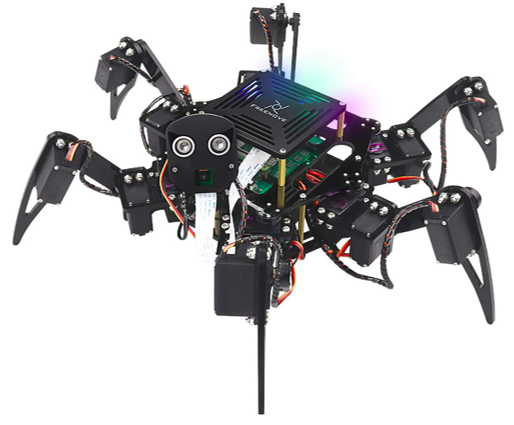
\includegraphics[scale=0.5]{figures/hexapod1.png}}
    \caption{The Freenove Big Hexapod robot kit}
    %\label{fig:Hexapod}
\end{figure}

%==========================================================================================
\section{Related Work}

\subsection{The Canonical SLAM Problem}
Given an accurate map of an environment, it is relatively straightforward to localize based on the features. Conversely, given accurate localization (for instance, by perfect dead reckoning), it is relatively straightforward to construct a map. However, taking neither as given turns this into a ``chicken and egg'' problem, called simultaneous localization and mapping (SLAM). In order to resolve this, we define a state vector of both the vehicle configuration and the observed landmarks thus far: \cite{corke}

\begin{equation*}
    \hat{\mathbf{x}} = (x_v,y_v,\theta_v,x_1,y_1,x_2,y_2, \ldots x_M, y_M)^T \in \mathbf{R}^{(2M+3) \times 1 }
\end{equation*}

The covariance estimate of this vector is:

\begin{equation*}
    \hat{\mathbf{P}} = \begin{bmatrix}
        \hat{\mathbf{P}}_{vv} & \hat{\mathbf{P}}_{vm} \\
        \hat{\mathbf{P}}_{vm}^T & \hat{\mathbf{P}}_{mm}
    \end{bmatrix}
\end{equation*}

wherein $\hat{\mathbf{P}}_{vv}$, $ \hat{\mathbf{P}}_{mm}$, and $\hat{\mathbf{P}}_{vm}$ are the covariances of the vehicle pose, landmark positions, and correlation between pose and landmarks, respectively. An extended Kalman filter can be used to predict and update the state and covariance.

New landmarks can be incorporated by extending the covariance matrix:
\begin{equation*}
    \hat{\mathbf{P}}\langle k \rangle ' = \mathbf{Y_z}\begin{bmatrix}
        \hat{\mathbf{P}} \langle k \rangle & 0\\
        0 & \hat{\mathbf{W}}
    \end{bmatrix} \mathbf{Y_z}^T
\end{equation*}

wherein $\hat{\mathbf{W}}$ is an estimate of the sensor covariance and $\mathbf{Y_z}$ is the so-called ``Insertion Jacobian", given by: \begin{equation*}
    \mathbf{Y_z} \equiv \frac{\partial \mathbf{y}}{\partial \mathbf{z}} = \begin{bmatrix}
        \mathbf{I}_{n \times n} & & \mathbf{0}_{n\times 2} \\
        \mathbf{G}_x & \mathbf{0}_{2\times n-3} & \mathbf{G}_z
    \end{bmatrix}
\end{equation*}

wherein $\mathbf{G}_z$ and $\mathbf{G}_x$ are the partial derivatives of the function $\mathbf{g}$ which gives the coordinates of an observed landmark based on known vehicle pose.

However, implementing SLAM requires a way to associate landmarks with locations in space. In the case of visual SLAM, feature recognition from a camera image is used to determine the landmarks to be used. This will be discussed further in the section below.

%------------------------------------------------
\subsection{ORB-SLAM}

\begin{figure}[H]
    \centering
    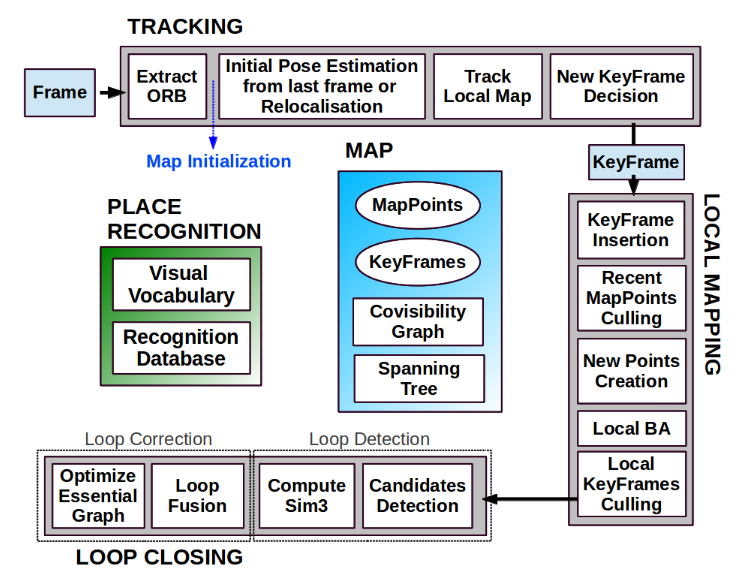
\includegraphics[width=\columnwidth]{figures/ORBSLAMoview.png}
    \caption{Overview of the ORB-SLAM system \cite{ORBSLAM}}
    \label{fig:OSLAMOview}
\end{figure}

The specific SLAM solution we implemented was the ORB-SLAM monocular visual SLAM algorithm, as proposed by Mur-Artal et. al. \cite{ORBSLAM} and summarized in Figure \ref{fig:OSLAMOview}.

In order to allow real-time performance without reliance on onboard GPUs or other co-processing units, ORB-SLAM bases its feature detection around so-called ``ORB features" as introduced by Ruble et. al. \cite{ORB} which are far less computationally expensive than SIFT or SURF detection.

The ORB-SLAM algorithm can be divided into three major sub-steps: tracking, local mapping, and loop closing, each of which is discussed in the following subsections.

%------------------------------------------------
\subsubsection{Tracking}

When a frame is input to the algorithm, first the ORB features are extracted. Next, these features are compared to the previous frame in order to estimate pose. Once this estimate is completed, the map is projected onto the new frame and we search for correspondences between the map and the frame. Finally, we decide if the current frame should be used as a keyframe going forward based on the number of points tracked, the similarity of those points to the previous keyframe, and the time since the last keyframe was spawned.

%------------------------------------------------
\subsubsection{Local Mapping}

This process is performed only if a new keyframe is added in the final step of the tracking process. First, the new keyframe is added to the covisibility graph and linked to the other keyframe which has the most points in common. Next, a bag of words representation for this keyframe is computed. After this, points in the map are tested to determine whether they are ``good enough'' to retain, or if they should be culled. This standard of ``good enough'' is determined based on two criteria. First, the algorithm predicts, from the position of the map point, in which other keyframes it should have been visible, and checks if it was visible in those frames. So long as it is found in over $25\%$ of them, it is not rejected. Second, it must also appear in at least three other keyframes, although this condition is skipped when first initalizing the map as it would otherwise prevent the inclusion of any points in the map.
Next, the ORB features from the new keyframe are triangulated with each of the connecting keyframes in the covisibility graph. For each unmatched ORB, we can simply search for matches within the set of unmatched ORBs in the other keyframes. Finally, a local bundle adjustment is performed to optimize the covisibility graph.
As an optional step, we can discard keyframes which have too many points in common with too many other keyframes. This can help to keep the model lightweight and reduce the processing required.

%------------------------------------------------
\subsubsection{Loop Closing}

With our new keyframe having been added in the previous step, we can now proceed to Loop Closing. Using the Bag of Words representation as previously calculated, we compare the similarity of the newest keyframe to each of its neighbors in the covisibility graph. The lowest of these similarities is saved. Any of the previous keyframes whose saved value is lower than that of our newest keyframe is retroactively discarded in order to improve robustness of the algorithm. Loop candidates must have three frames in a row which are mutually consistent.

We first compute ORB correspondences between the current keyframe and the loop candidates, which give 3D to 3D correspondences. We use these results to fuse the duplicated map points and insert new edges into the covisibility graph. The new keyframe is corrected with a similarity transform, and this correction is propagated to the keyframe's neighbors in the covisibility graph. Map points seen by the loop keyframe are similarly projected into the new keyframe that is being added and its neighbors. Any matches found in this projection are subsequently fused and all keyframes with fused map points have their edges updated correspondingly, thus concluding the loop closure and the ORB-SLAM algorithm.

%==========================================================================================
\section{ Method }

The hardware, coordinate frames, and algorithms used are discussed in this section.

%-----------------------------------------------------------------------------------
\subsection{ Hardware }

 This project implements SLAM on a real hexapod robot platform. This platform is built of discrete components, including the hexapod hardware, sensors, and processors.

%------------------------------------------------
\subsubsection{ Hexapod }

This project uses the Freenove Big Hexapod kit as the hardware base. This kit comes with a six-legged robot chassis, where each leg has three degrees of freedom (DOF) that can be individually controlled. Each joint is actuated by an individual MG-996R servo motor, which can be commanded to move between $0-180^{\degree}$ given a 50 Hz pulse width modulation (PWM) signal. To manage communication to all 18 leg servos, the servos are controlled by the PCA9685 servo driver module, which has a standard Python library to allow software control of the PWM signals.

%------------------------------------------------
\subsubsection{ Processor }
The Raspberry Pi (RPi) 4 acts as the main processor of the robot assembly.  The RPi's CPU is a Broadcom BCM2711B0 with stock clock speeds of 1.5GHz, which has been over-clocked to 1.9 GHz for improved performance.  The model RPi used in this project includes 8MB of DDR RAM. A heat sink and active fan are used to keep CPU temperatures manageable during strenuous processing. The RPi is also setup to boot from an external SSD connected through USB 3.0, rather than the typical SD card boot hardware; this improves read-write speed and boot times.

\begin{figure}[H]
    \centerline{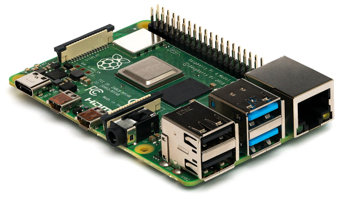
\includegraphics[scale=0.8]{figures/pi1.png}}
    \caption{The Raspberry Pi 4 single-board computer}
    \label{fig:raspberry_pi}
\end{figure}

%------------------------------------------------
\subsubsection{ Seeker Gimble }

The Freenove Big Hexapod kit comes equipped with two additional sensors used for this project: an ultrasonic range sensor and a camera. These sensors are mounted together on a two-axis gimble called the ``seeker.'' The seeker can be pointed in azimuth and elevation directions individually by two MG90S servo motors, which are controlled by the RPi similar to the leg servos.

%------------------------------------------------
\subsubsection{ Raspberry Pi Camera Module}

A Raspberry Pi OV5647 infared night vision camera module is mounted to the seeker and is optimized for use with the Raspberry Pi.  It connects via a dedicated ``camera module port'' on the RPi's PCBA. It can be used for both still photos and video, and is the primary sensor for this project.

\begin{figure}[h]
    \centering
    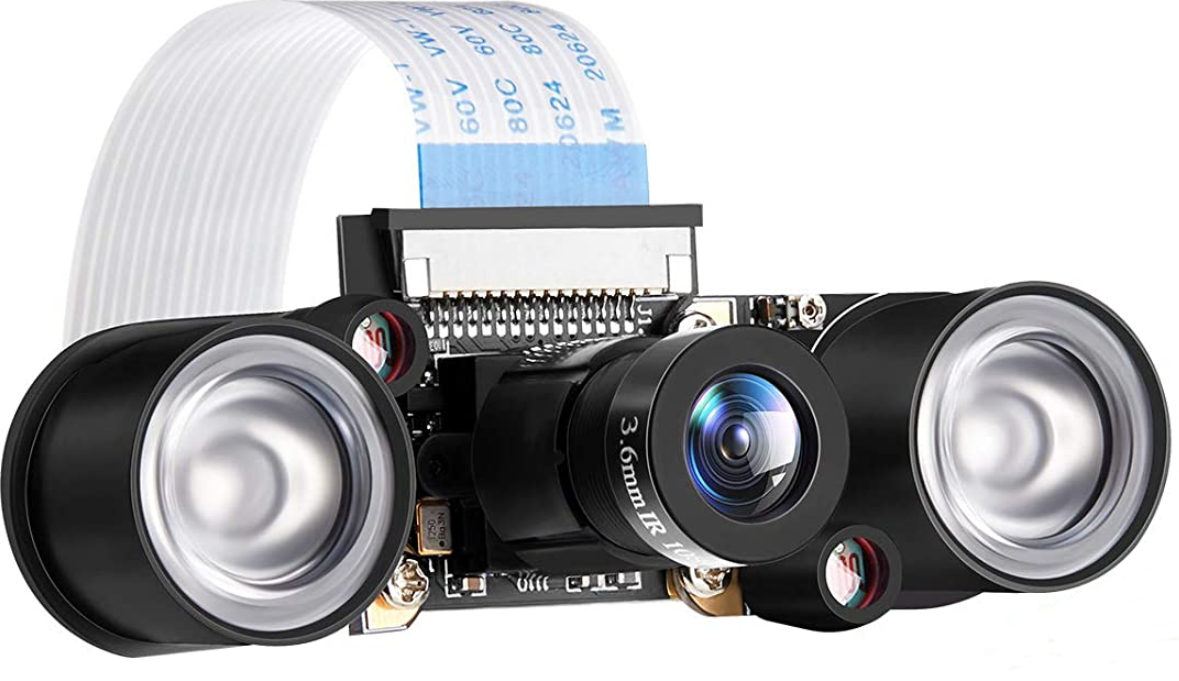
\includegraphics[scale=0.15]{figures/camera.png}
    \caption{Raspberry Pi OV5647 infared nigh vision camera module}
    \label{fig:raspberry_pi_cam}
\end{figure}

%------------------------------------------------
\subsubsection{ Inertial Measurement Unit (IMU)}
The MPU-6050 is an affordable, OTS inertial measurement unit (IMU) that is capable of providing linear acceleration, angular velocity, and temperature measurements to the Raspberry Pi at 50 Hz \cite{mpu6050}.  The IMU is hard-mounted to the motor driver board and is located just underneath the RPi. The IMU connects to the RPi via I\textsuperscript{2}C on the RPi's GPIO module.

This low-cost IMU presents inconsistent bias values for each signal which must be removed to prevent pose estimation drift. To perform this, a calibration routine was implemented in the IMU node at initialization, which assumes the robot body is static and level with the ground. The sensor is polled for some fixed time period (0.5s), and an average of all readings from both the accelerometer and gyroscope is computed. Gravitational acceleration of $9.81 m/s^2$ is removed from the $\hat{z}$ component of the accelerometer. These bias values are then removed from all future IMU measurements before publishing the data out as a ROS topic.

%------------------------------------------------
\subsubsection{ Desktop Computer }
To aleviate the computational burden of ORB-SLAM3 on the RPi, the distributed processing capabilities of ROS1 were exploited for this project by using a desktop computer to supplement the processing. This computer contained an AMD Ryzen 7 3800X 8-core CPU, an Nvidia RTX 2060 Super graphics processor, and 32Gb of onboard RAM running Ubuntu 20.04. The RPi ran all hardware-dependent ROS nodes, including the camera and IMU sensor nodes and the servo actuator nodes. All other ROS nodes, the ROS core, and any extra analysis tools, were run on the desktop machine. Communication was handled wirelessly using the local network WiFi.

%------------------------------------------------
\subsection{ Sensor Calibration }
To effectively use the sensors, they first needed to be calibrated. The approaches used are discussed below.

\subsubsection{ Camera }
To calibrate the embedded camera with intrinsic hardware parameters, the open-source camera\_calibration ROS package was used \cite{cameracalibration}. This package contains a ROS node that subscribes to a camera video topic of type sensor\_msgs/Image \cite{imagemsg}. Users present a grid of known shape and dimension to the camera at different poses across the whole image field of view, as seen in Figure \ref{fig:camera_calibrate}. Once enough data is collected, the tool runs an optimization routine to calculate camera properties like focal length and distortion characteristics.

\begin{figure}[H]
    \centerline{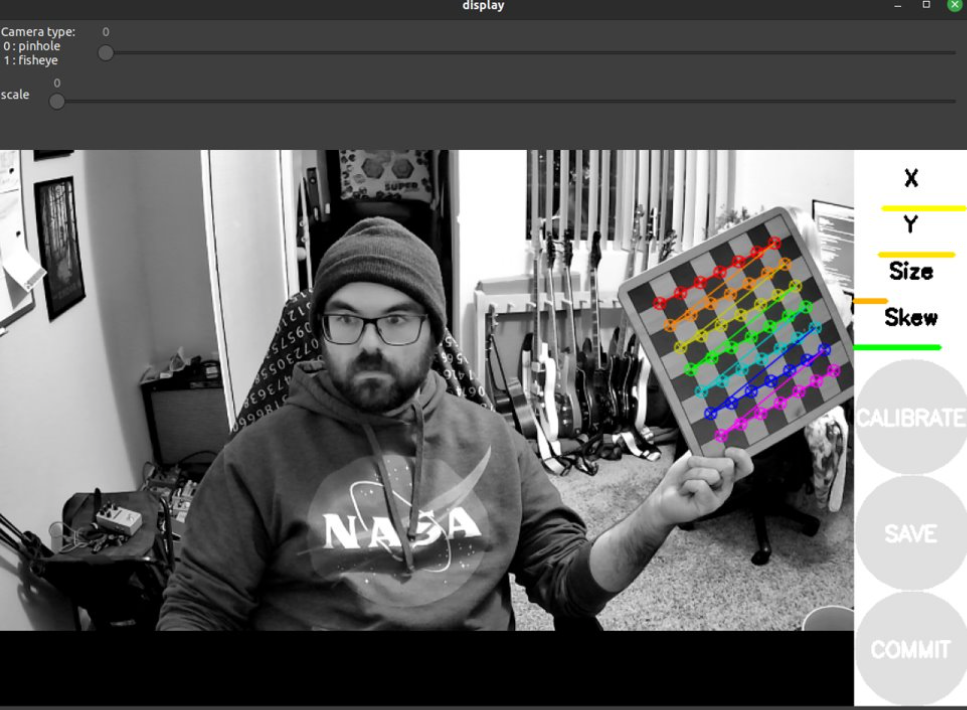
\includegraphics[scale=0.27]{figures/camera_calibrate.png}}
    \caption{ camera\_calibration GUI detecting a 7x7 checkerboard grid of known dimensions}
    \label{fig:camera_calibrate}
\end{figure}


%-----------------------------------------------------------------------------------
\subsection{ Coordinate Frames }

Several right-handed coordinate frames are defined and used throughout this project:

\begin{itemize}
    \item The odometry frame is used as the world-fixed coordinate frame. Both the extended Kalman filter (EKF) and the ORB\_SLAM3 algorithm estimate pose relative to this frame.

    \item The ground frame is placed under the robot body frame and is a child of the odometry frame. Desired foot positions for the walking gait are calculated in this frame, since motion is dependant on foot contact with the ground rather than relative to the robot body.

    \item The robot body frame is static relative to the hexapod chassis hardware and is referenced relative to the ground frame. The $\hat{x}_b$ direction points forward, the $\hat{y}_b$ direction points left (port side) of the body, and the $\hat{z}_b$ direction points straight up. This coordinate frame is located in the center of the robot belly such that this frame contacts and is parallel to the ground when $z_b = 0$.

    \item The seeker frame is kinematically linked to the body via a two axis gimble, with the $\hat{x}$ direction pointing out from the seeker. The camera is statically mounted on the seeker, with its own coordinate frame whos $\hat{z}$ direction points out from the seeker and the $\hat{x}$ direction points to the robot starboard side. The transformation from body to camera frame is a function of seeker azimuth and elevation servo angles. Because the seeker gimble servos do not give encoder data back to the RPi, it is assumed that commanded joint angles are the true joint angles. This transformation is calculated as follows.

    \[
    T^b_c = T^b_n T^n_{az} T^{az}_{el} T^{el}_{c}
    \]

    \[
    T^b_n = \begin{bmatrix} 0 & -1 & 0 & 0 \\
                            1 & 0 & 0 & 0.0762 \\
                            0 & 0 & 1 & 0.1386 \\
                            0 & 0 & 0 & 1 \end{bmatrix}
    \]
    \[
    T^n_{az} = \begin{bmatrix} \cos{az} & 0 & \sin{az} & 0 \\
                               \sin{az} & 0 & -\cos{az} & 0 \\
                               0 & 1 & 0 & 0 \\
                               0 & 0 & 0 & 1 \end{bmatrix}
    \]
    \[
    T^{az}_{el} = \begin{bmatrix} \cos{el} & 0 & -\sin{el} & L \cos{el} \\
                                  \sin{el} & 0 & \cos{el} & L \sin{el} \\
                                  0 & -1 & 0 & 0 \\
                                  0 & 0 & 0 & 1\end{bmatrix}
    \]

    \[
    T^{el}_{c} = \begin{bmatrix} 0 &  0 & 1 & 0 \\
                                 0 & -1 & 0 & 0.0167 \\
                                 1 &  0 & 0 & 0 \\
                                 0 &  0 & 0 & 1 \end{bmatrix}
    \]

Where $L$ is the length of the gimble, and $az$ and $el$ are the azimuth and elevation angles, respectively. All angles are given in radians, and distance is given in meters.

\end{itemize}

\begin{figure}[h]
    \centering
    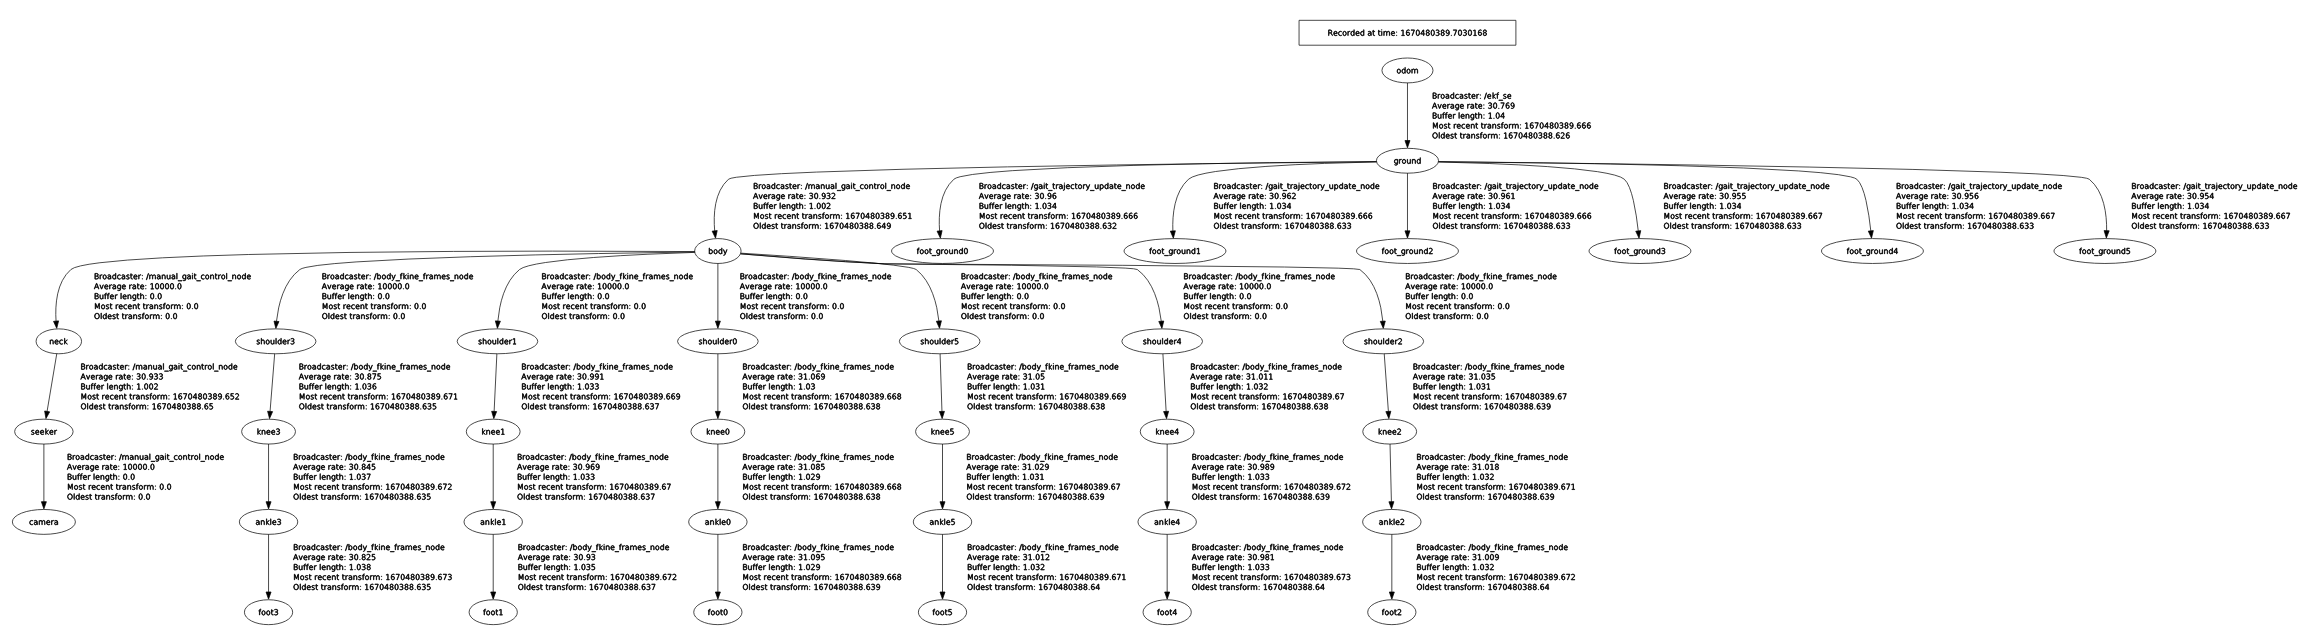
\includegraphics[scale=0.11]{figures/tf_tree.png}
    \caption{ ROS tf2 \cite{tf2} kinematic transformation tree, including all leg-related frames }
    \label{fig:tf_tree}
\end{figure}

%-----------------------------------------------------------------------------------
\subsection{ Software Architecture }

The RPi embedded on the robot runs Ubuntu Mate 20.04 as the operating system. All control software for the robot is written as ROS1 Noetic nodes, written in Python and C++. Nodes are broken up between hardware control, gait manipulation, and analytical or sensor processing. An RQT ROS node graph can be seen in Figure \ref{fig:rqt}.


\begin{figure}[h]
    \centering
    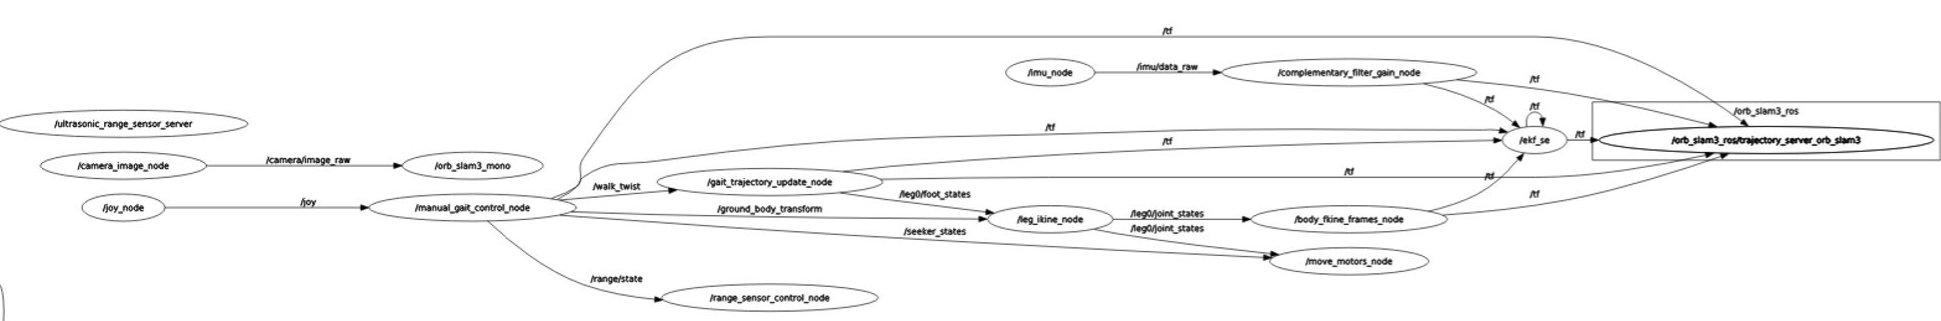
\includegraphics[scale=0.12]{figures/rosgraph.png}
    \caption{ Node design for ROS software architecture }
    \label{fig:rqt}
\end{figure}

In order to facilitation motion through the space we wish to map, a master controller node receives input from an Xbox controller to determine the desired body motion. This node outputs a twist vector and a body pose relative to the ground, as well as seeker gimble angles. The gait update node receives the twist vector and calculates new desired foot positions. An inverse kinematics node then calculates new joint angles, which are received by the motor driver node to actuate the servo motors.

\subsubsection{ Extended Kalman Filter (EKF)}

For continuous body pose estimation, the robot\_localization ROS package \cite{robotlocalization} was used to implement an extended Kalman filter (EKF). This filter receives the commanded twist vector in the ground frame, as well as IMU sensor data in the body frame, and estimates the robot's pose relative to the fixed odometry frame over time.

\subsubsection{ ORB-SLAM3 Node}

A fork of the ORB-SLAM3 library was used for this project \cite{orb_slam_ros}. This package modifies the original ORB-SLAM3 library to streamline interfacing it with ROS1 Noetic. An additional ROS wrapper repository was also used to call the ORB-SLAM3 algorithm as a ROS node \cite{orb_slam_ros_wrapper}. This wrapper was modified for this project to publish the camera pose as a ROS PoseStamped messages \cite{posestamped} and the map as a ROS PointCloud2 message \cite{pointcloud2} when the algorithm maintains a track on the map. The node accpets a configuration YAML file with parameters, including the calibrated camera properties, camera framerate, and internal settings for the ORB-SLAM3 algorithm. This node subscribes to the camera data published by the robot.


%==============================================================================
\section{Experiment}

The robot was placed in an unobstructed environment with objects to detect of different colors and shapes. The desktop computer started the ROS core, and the robot processor connected to this core. The robot then booted up the hardware sensor and actuator nodes, and the desktop computer kicked off all other ROS nodes, including the ORB-SLAM node. The user then commanded the robot to move around the room using an Xbox controller. As video data transmits from the camera mounted on the robot to the desktop computer, the ORB-SLAM3 node processed the data and outputs a point map of the environment and the estimated robot pose. Simultaneously, the IMU data and the commanded twist vector were used to estimate the robot pose in the EKF.

%==============================================================================
\section{ Results}
The ORB-SLAM algorithm has been successfully implemented on the hardware, adapted for ROS using C++ as the main programming language. The robot can identify key points in video data as seen in Figure \ref{fig:keypoints} and generate a map of the environment as it moves through it. The results of this mapping can be seen in Figure \ref{fig:map} below.

%% TODO: Add figure showing constructed map from ORB-SLAM

\begin{figure}[h]
    \centering
    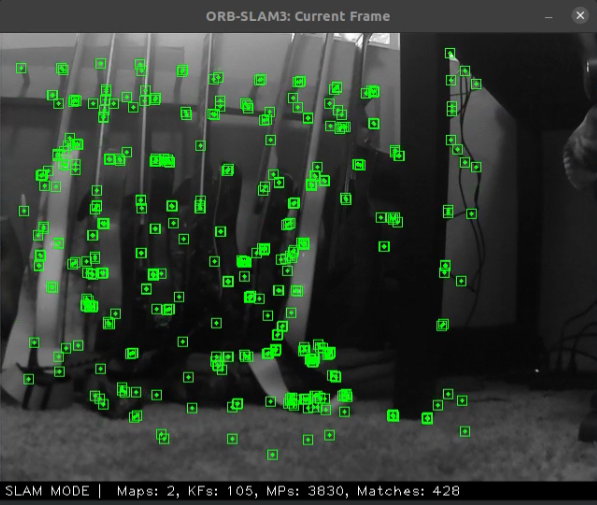
\includegraphics[scale=0.4]{figures/orb_slam3_keypoints.png}
    \caption{Example key points identified in ORB-SLAM3 from video feed}
    \label{fig:keypoints}
\end{figure}

\begin{figure}[h]
    \centering
    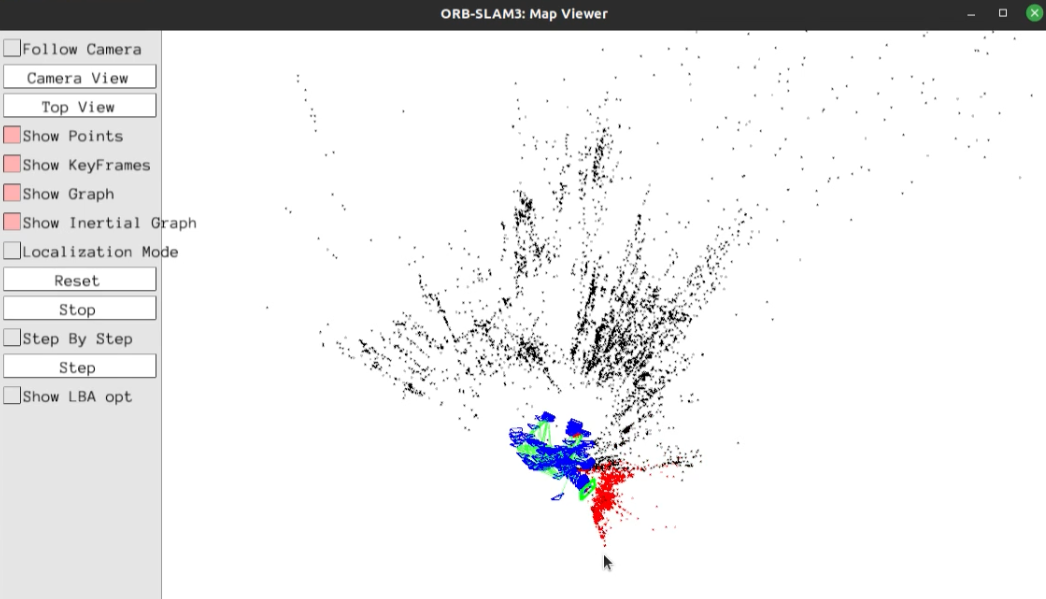
\includegraphics[scale=0.24]{figures/orb_slam3_map.png}
    \caption{ Generated Map from the Hexapod's Measurements}
    \label{fig:map}
\end{figure}

An example of the pose estimation generated from ORB-SLAM3 and the EKF can be seen in Table \ref{table:pose_data}. Truth data is obtained by measuring the true motion of the robot relative to its initial position using a tape measure. 

\begin{table}[h!]
\begin{adjustbox}{width=0.5\textwidth}
\begin{tabularx}{0.6\textwidth}{ ||c c c c c c c c ||}

    \hline
    Source & $p_x$ & $p_y$ & $p_z$ & $q_w$ & $q_x$ & $q_y$ & $q_z$ \\
    \hline \\
    Truth & -0.762 & -1.320 & 0.212 & 0.5 & 0 & 0 & -0.867 \\
    EKF & -0.6 & -0.239 & -0.822 & -0.005 & -0.007 & -0.216 & 0.976 \\
    SLAM & 0.166 & 0.030 & -0.069 & -0.011 & 0.713 & -0.153 & 0.684 \\
    \hline

\end{tabularx}
\end{adjustbox}
\caption{Pose estimation for SLAM and EKF systems}
\label{table:pose_data}
\end{table}

%=========================================================================================

\section{ Discussion }

Our implementation of the ORB-SLAM algorithm onto the hexapod is able to successfully create a map of its surrounding environment. The room is shown in Figure \ref{fig:room}. Evaluating this map by visual inspection, we are able to distinguish several elements of the scene which have been constructed in the map, for instance the set of guitars along one wall of the room, the closet to the left, and the hallway to the right. Because of our lack any known-good map (due to use of real, in person measurements rather than public datasets), we are unable to make quantative statements about the accuracy of the map points that we have generated. However, it is clear that the generated map is noisy and would be difficult to use in a practical implementation, without some other information like another map of the environment known \emph{a proiri}.

\begin{figure}[h]
    \centering
    \includegraphics[scale=0.04]{figures/room_pan.jpg}
    \caption{ Panoramic image of the mapped environment }
    \label{fig:room}
\end{figure}

One significant drawback of this implementation was the difficulty in obtaining and maintaining a track of the map. The camera needs to move before the first SLAM map is initialized, which means the first pose estimation from SLAM is in disagreement with the near-continuous EKF pose estimate that begins tracking immediatley. As the camera explores new areas, it was easy to lose track and drop the map again, resulting in periods where no SLAM-based pose estimation is available. The poor frame rate of the video most likely caused this, but this is a fixed hardware limitation with our implementation. When features are detected again, a new map is generated, reinitializing the pose estimate with discontinuities relative to the EKF pose. Only when loop closure occurs and maps are merged does the SLAM pose estimation snap back to the initial track. Autonomous systems typically require a smooth, continuous pose estimation approach, and ORB-SLAM would need a lot of accomidations to achieve this in a practical application.

Despite the discontinuities, the orientation estimation of SLAM appeard reasonably accurate relative to where the map initializes, especially in comparison to the estimation generated by the EKF. The EKF was prone to large drifts over time, particularly in the $\hat{z}$ direction. This is most likely due to the jittery nature of the walking gait, causing large spikes in accelerometer data that drives the EKF off truth. SLAM, on the other hand, showed responsive pose updates in response to camera motion, especially when lots of features were being tracked in the map. However, the magnitude of translation for the SLAM-generated pose estimation was off; only small translations are shown relative to the truth. A fusion of the two state estimation approaches would be benificial for practical implementation. Maintaining an EKF for each map generated by SLAM that uses the commanded twist vector, IMU data, and SLAM-based pose estimation may be a viable solution to provide continuous state estimation while taking advantage of the localization that SLAM provides. Using an external distance measurement like a range sensor may also supplement the poor scaling inherent in monocular VSLAM. 

%=========================================================================================
\printbibliography

\end{document}
